\documentclass[12pt]{article}
\usepackage{graphicx, amsmath, hyperref, amssymb}
\usepackage{subcaption}
\usepackage{algorithm}
\usepackage{algpseudocode}
\graphicspath{ {./} }
\setlength{\oddsidemargin}{0.25 in}
\setlength{\evensidemargin}{-0.25 in}
\setlength{\topmargin}{-0.6 in}
\setlength{\textwidth}{6.5 in}
\setlength{\textheight}{8.5 in}
\setlength{\headsep}{0.75 in}
\setlength{\parindent}{0 in}
\setlength{\parskip}{0.1 in}

\begin{document}
\thispagestyle{plain}
   \newpage
   \setcounter{page}{1}
   \noindent
   \begin{center}
   \framebox{
      \vbox{\vspace{2mm}
    \hbox to 6.28in { {\bf BioE 131: Intro to Computational Biology}
                        \hfill Fall 2020 }
       \vspace{4mm}
       \hbox to 6.28in { {\bf \Large \hfill RNA Folding  \hfill} }
       \vspace{2mm}
       \hbox to 6.28in { {\it Professor: Ian Holmes \hfill} }
      \vspace{2mm}}
   }
   \end{center}
   {Notes written by Vikram Shivakumar}
   \vspace*{4mm}


\section{Introduction}
{\bf RNA structure} is an important area of computational biology, and the ability to predict structure, folding kinetics, and other properties of RNA molecules is important to understanding processes like translation and transcriptional regulation. In these notes, we will cover some algorithms for RNA structure prediction, as well as a motivating example for using them, RNA logic circuits.

\subsection{Background}
RNA sequences are composed of 4 nucleotides, {\bf A}denine, {\bf G}uanine, {\bf C}ytosine, and {\bf U}racil. These nucleotides form base pairs as in DNA, with 4 possible combinations: A-U U-A, G-C, and C-G. In RNA, another set of {\bf wobble base pairs} can form: G-U and U-G. Other combinations of nucleotide base pairs can also occur in RNA with rare frequency (in cases where the base pair is required for overall molecule stability or in cases of mutation). One important aspect of base pairing to note is the strength of the hydrogen bonding in the base pair. G-C pairs contain 3 hydrogen bonds, while A-U and G-U pairs only contain 2, so G-C base pairs are relatively more stable.
Base pairing in RNA molecules can lead to various structural features in the overall molecule.
\begin{figure}[h]
    \centering
    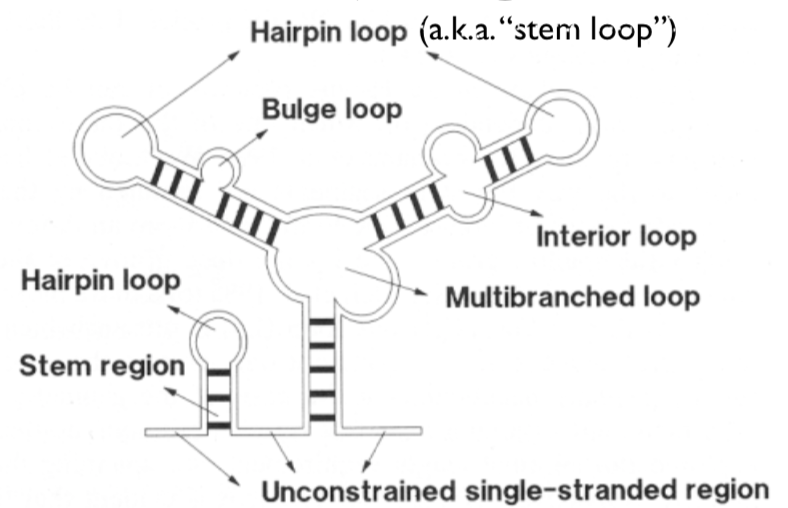
\includegraphics[height=1.8in]{rna_loop}
    \caption{Examples of loop regions in RNA}
    \label{fig:loop}
\end{figure}

\subsection{Folding Energetics}
The primary energetic interactions in RNA structure are base pairs, but there are more factors to consider when calculating the free energy of an RNA molecule. One example is {\bf base pair stacking}: multiple adjacent base pairs which can affect the overall stability of the structure through various interactions. {\bf Van der waals} forces between adjacent bases and \textbf{steric interactions} between the backbones of the chains can affect the stability of the stacked base pairs. Another factor is effect of stacking the \textbf{delocalized pi orbitals} present in the aromatic ring structures of adjacent nucleotides.\\[10pt]
The combinations of these various factors makes it difficult to predict folding energy from individual base pairs, but by empirically measuring the folding energies of different RNA sequences, the energies of different base pair combinations can be estimated. To determine the folding of an RNA polymer, we need to consider the molecule's \textbf{free energy}. A polymer that folds back on itself has lower entropy than a polymer in which all conformations is allowed (conceptually, "the number of random walks that return home" is less than "the number of random walks that do not return home"), so to determine folding we need to consider free energy which encompasses both \textbf{entropy} and energy (the non-entropy component of free energy sometimes called \textbf{enthalpy}).  \\[10pt]
Some stretches of base pairing can contain interrupting unpaired bases, which leads to the formation of loops and bulges. These features can also contribute to the overall stability of the molecule, as the size of the loops and bulges constrain the overall conformation. Certain loops (like tetraloops and triloops), as well as certain bulges are more favorable than others, contributing to the overall folding free energy.

\section{RNA Logic}
One goal in synthetic biology is to engineer biological circuits, similar to electronic circuits, in genetic systems. To achieve a circuit-type mechanism, a few components are necessary: inputs, processing (like logic gates), and outputs. The following example will discuss a method for creating RNA circuits, one of many motivations for RNA structure prediction.

\subsection{Biological I/O}
There are a few components necessary to build logical circuits from RNA. First we need some sort of input mechanism that can convert an input signal into the input for the logic gate. {\bf Aptamers} are structured RNA and DNA molecules that form binding pockets for specific ligands. These aptamers can generated by {\it in vitro} selection on a specific ligand, which serves as the input to the circuit. One example of a naturally occuring RNA aptamer is the {\bf riboswitch}. These RNA molecules form binding pockets for metabolites, and in turn can effect transcription and translation, and even trigger self-cleavage.\\[10pt]
The most common output in this scenario is {\bf Green Fluorescent Protein (GFP)}, which contains a chromophore that produces a green fluorescence. Using GFP makes detecting the output as simple as seeing the presence of green fluorescence.
\subsection{Ribozymes}
Finally, to create logic circuits, we need logic gates like AND, OR, and NOT. One method for creating logic gates in biological systems was proposed in 2005 by Penchovsky and Breaker (\href{https://dx.doi.org/10.1038/nbt1155}{read the full paper here}). They devised a system that uses a variation on the {\bf hammerhead ribozyme}. A ribozyme is an RNA molecule that catalyzes a reaction, for example peptide bond formation (ribosomes) or phosphodiester bond cleavage/formation (RNase P, self-splicing introns, etc).\\[10pt]
The hammerhead ribozyme is able to catalyze self-cleavage in the right secondary structure conformation. Penchovksy and Breaker were able to induce self-cleavage in these ribozymes by causing allosteric shifts in secondary structure, which in turn creates the correct conformation for self-cleavage. They accomplished this by modifying the ribozyme with an oligonucleotide binding site (OBS) which when bound, causes the ribozyme structure to form.
\begin{figure}[h!]
    \centering
    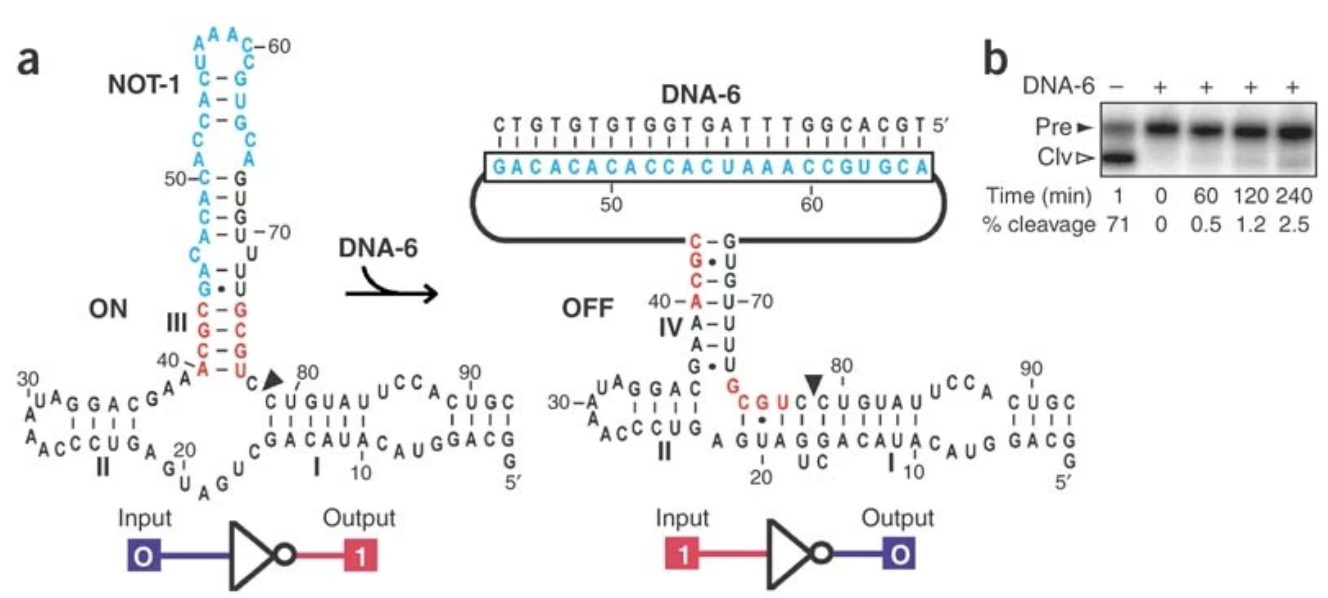
\includegraphics[width =.9\linewidth]{notgate.png}
    \caption{NOT gate [from Penchovsky and Breaker (2005)]}
    \label{fig:not_gate}
\end{figure}\\
An example of a NOT gate implemented using a hammerhead ribozyme is shown in Figure \ref{fig:not_gate}. The three loops (I, II, III) constitute the ribozyme and are necessary for self-cleavage. When the complementary DNA sequence to the OBS (shown in blue) is present, a conformation change occurs which disrupts the ribozyme portion of the molecule, halting self-cleavage (turning the gate OFF).\\[10pt]
Similarly in the AND and OR gates, there are 2 oligonucleotide binding sites. In the case of the AND gate, complementary binding to both sites causes a conformational change which leads to the hammerhead ribozyme and self-cleavage. For the OR gate, only complementary binding to one OBS is necessary to form the ribozyme. Thus, the presence of a cleaved portion of the ribozyme indicates that the gate is active, and vice-versa.
\begin{figure}[ht]
    \centering
    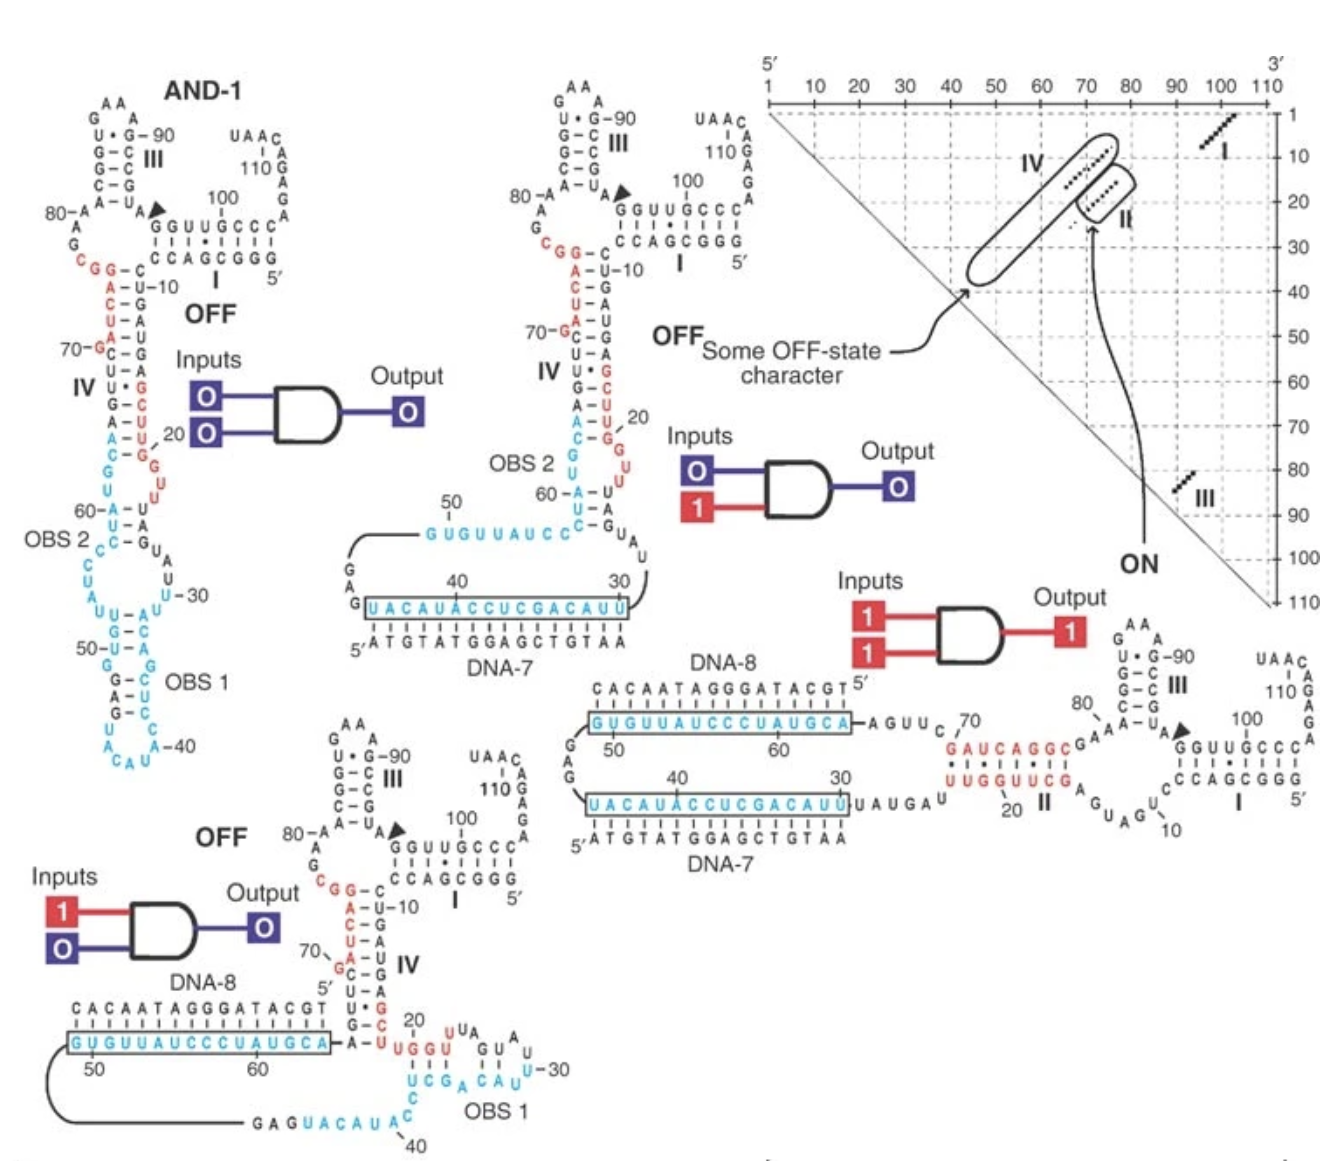
\includegraphics[width =.8\linewidth]{andgate.png}
    \caption{AND gate [from Penchovsky and Breaker (2005)]}
    \label{fig:and_gate}
\end{figure}\\
One thing to note in Figure \ref{fig:and_gate} is the graph on the top right, called a {\bf McCaskill dotplot}. The axes of the plot contain the indices of each base in the RNA sequence. A point at position $(i, j)$ in the dotplot represents the presence of a basepair between the bases at positions $i$ and $j$. The brightness of the dot represents the probability of the base pair occurring (we will discuss how to calculate these probabilities later in the note).\\[10pt]
Seelig, Winfree, {\it et al} proposed another example of RNA based logic circuitry in 2006. Their mechanism relies only on strand displacement and sequence complementarity, meaning the gates are reversible (no cleavage necessary!). 
\section{Algorithms for RNA Folding}
To design RNA structures like ribozymes and riboswitches, we need a few computational tools for tasks like structure prediction, predicting folding kinetics, and visualizing RNA structure. Now we will cover some algorithms and methods for predicting folding kinetics and structure from an RNA sequence.

\subsection{Nussinov Algorithm}
The Nussinov algorithm addresses the following problem: ``{\it Given an RNA sequence, determine the maximum number of strictly-nested Watson-Crick basepairs it can form}". The algorithm solves this problem using a technique called {\bf dynamic programming}. Dynamic programming involves breaking a problem into multiple subproblems recursively, and solving them in order, building up to the final solution.\\[10pt]
Let's take a look at how the algorithm works. Given a sequence $X$ with the best foldback structure $S$, one of the following must be true: 
\begin{enumerate}
    \item the terminal bases on each end of the sequence are paired\\[9pt]
    OR
    \item there is at least one {\it bifurcation} in $S$ (where each side of the split has strictly nested foldback structure)
\end{enumerate} 
In case 1) we can remove the terminal bases which are paired, and find the optimal foldback structure of the remaining sequence. In case 2) we can split the sequence into two at the bifurcation, and find the optimal foldback structure of each side. In both cases, we have broken down the problem into \textbf{subproblems}.

\begin{figure}[h]
    \centering
    \begin{subfigure}[b]{.45\textwidth}
    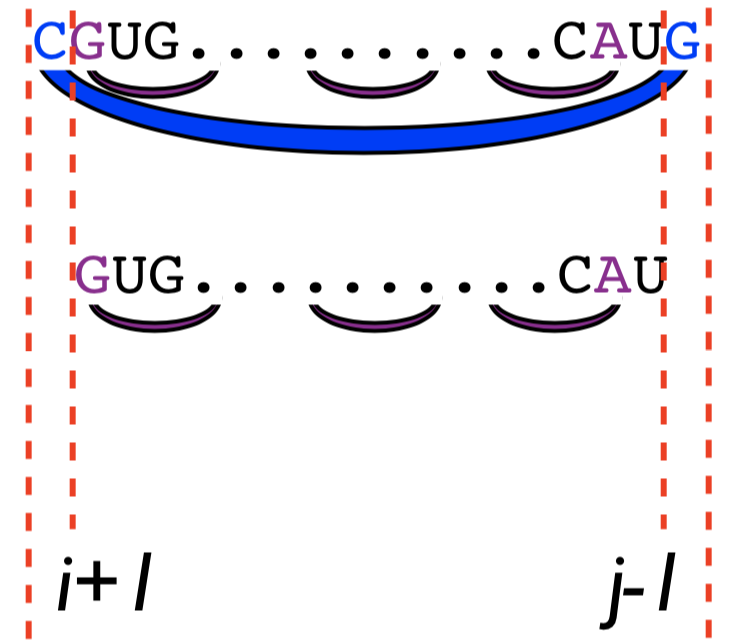
\includegraphics[width=\textwidth]{case1.png}
    \caption{Case 1}
    \end{subfigure}
    \hfill
    \begin{subfigure}[b]{.45\textwidth}
    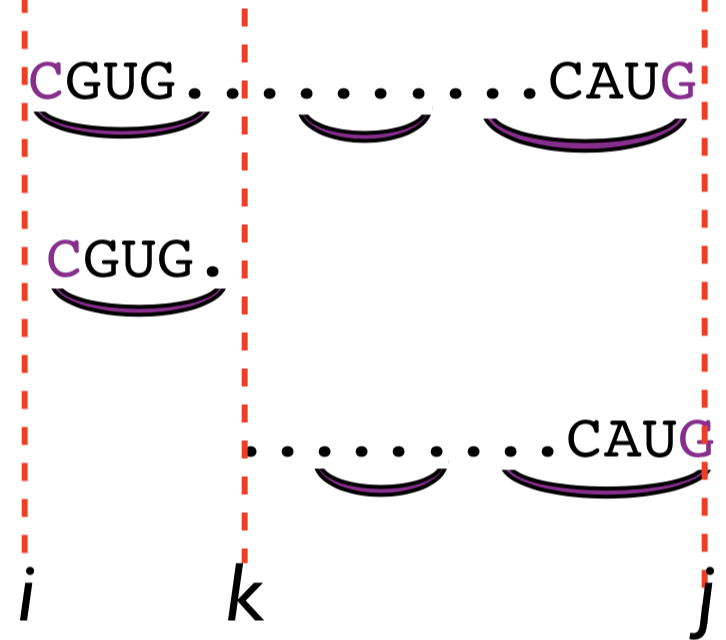
\includegraphics[width=\textwidth]{case2.png}
    \caption{Case 2}
    \end{subfigure}
    \caption{Splitting the problem into subproblems in both cases of the Nussinov algorithm}
    \label{fig:cases}
\end{figure}
We can formulate this in an equation, where $N_{ij}$ refers to the number of base pairs in the foldback structure of the subsequence from $i$ to $j$:\\[10pt]
\begin{equation*}
N_{ij} = \begin{cases}
N_{i+1, j-1} + 1 &\text{Case 1}\\
N_{ik} + N_{k+1,j} &\text{Case 2}\\
\end{cases}
\end{equation*}\\[10pt]
where $k$ is some index that represents the bifurcation of the sequence.\\
We can generalize these two cases a bit more:\\[10pt]
\begin{equation*}
N_{ij} = \begin{cases}
N_{i+1, j-1} + \delta_{WC}\left( X_i, X_j\right) &\text{Case 1}\\
\max\limits_{i\leq k <j}\left( N_{ik} + N_{k+1,j}\right) &\text{Case 2}\\
\end{cases}
\end{equation*}
$$\delta_{WC}\left(a, b\right) = \begin{cases}
1 & \text{if } a,b \text{ are complementary}\\
0 & \text{if } a,b \text{ are not complementary}
\end{cases}$$\\[10pt]
To decide which case to use for a sequence, we can compute both and take the case which maximizes the base pair count, similar to how we take the max over the possible splits in case 2. This yields the final equation for the Nussinov algorithm:\\[10pt]
\begin{equation*}
N_{ij} = 
\begin{cases}
\max 
\begin{pmatrix}
N_{i+1, j-1} + \delta_{WC} \left(X_i, X_j\right) \\
\max\limits_{i\leq k <j} \left(N_{ik} + N_{k+1,j}\right) 
\end{pmatrix}&\text{if } j > i\\
0&\text{if } j\leq i\\
\end{cases}
\end{equation*}\\[10pt]
where $N_{1, L}$ is the foldback structure for the entire sequence.\\[10pt]
Now that we've deconstructed the main problem into multiple subproblems, we need to solve the subproblems in order to build towards the final solution. Each problem should only use subproblems which we have already solved. 
The following pseudocode computes the final solution (and all intermediate subproblem solutions) in order:
\begin{algorithm}
\caption{Nussinov algorithm}
\begin{algorithmic}
\For{i = L to 1}
    \For{j = i to L}
        \State $N_{ij} \leftarrow N_{i+1, j-1} + \delta_{WC}\left(X_i, X_j\right)$
        \For{k = i to j-1}
            \State $N_{ij}\leftarrow max\left(N_{ij}, N_{ik}+N_{k+1, j}\right)$
        \EndFor
    \EndFor
\EndFor
\end{algorithmic}
\end{algorithm}\\
\subsection{Big O Complexity}
To describe how long the Nussinov algorithm takes to run, we need to use \textbf{Big O notation}. Big O notation describes the \textit{asymptotic} behavior, or how the algorithm scales on very large datasets. We are often only interested in \textit{order of magnitude} differences between algorithms, so we are not describing how long the algorithm takes, but how fast the runtime will grow if we increase the input size.\\[10pt]
Take for example the task of comparing each item in a list to every other item. The number of comparisons would be $N(N-1)/2$. To write this in Big O notation, we can ignore any constant factors, and only focus on the \textit{highest power} term. The reason for this is when the input size is very large, the smaller terms don't matter nearly as much as the highest powered term, so we can say it \textit{dominates}. Thus we can say there are on the \textit{order of} $O(N^2)$.\\[10pt]
The formal definition of Big O complexity is the following:\\
For a function $f(x)$ and $g(x)$, if $f(x) = O(g(x))$, then there exists some values $x_0$ and $C$ where the following holds:
$$|f(x)| \leq Cg(x) \text{ for } x\geq x_0$$
This means for \textit{sufficiently} large values of $x$, $f(x)$ is bound by a constant multiple of $g(x)$, meaning $f(x)$ grows asymptotically on the order of $g(x)$.\\[10pt]
Here are some common Big O formulae and their ordering:
$$O(N!) > O(2^N) > O(N^3) > O(N^2) > O(N\log N) > O(N) > O(\log N)$$

\subsection{Runtime of Nussinov Algorithm}
Looking at the pseudocode for the Nussinov algorithm, we see there are 3 for loops, and in each iteration, we are performing a constant number of iterations operation, so the time complexity is \textbf{$O(N^3)$}. This means if we increase the size of the RNA we are folding, the algorithm runtime will increase by a factor of $N^3$. What about the memory complexity? How much memory does the algorithm need? During the algorithm, we store values for each pair of indices $i, j$, representing optimal number of base pairs in the RNA sequence from $X_i$ to $X_j$. This means we are considering all combinations of indices, which as we've seen before is $O(N^2)$.
\subsection{Partition Function}
\label{partition}
In the beginning of the note, we discussed how the number of base pairs is not the only factor that contributes to a stable secondary structure, but using empirical data we can estimate the overall energy of a structure. Thus we need an algorithm that accounts for energy differences between structures, not just the number of base pairs.\\[10pt]
RNA folding is a thermodynamic process, with each structure $S$ associated with an energy $E_S$. In a thermodynamic equilibrium, the probability of a structure is proportional to the \textbf{Boltzmann factor}: $e^{-\beta E_S}$, where $\beta = \frac{1}{k_BT}$ ($k_B$ is the Boltzmann constant and $T$ is the temperature). To compute the actual probability of the structure, we need to scale the Boltzmann factor so the probabilities of every possible structure sum to 1. The scaling term is called the $partition function$, and is the sum of the Boltzmann constant for every possible structure:
$$Z\left(X\right) = \sum_{S\in \mathbb{S}(X)}e^{-\beta E_S}$$
where $\mathbb{S}(X)$ is the set of possible structures for sequence $X$. Thus the probability of a structure S is given by:
$$P(\text{structure } S | \text{sequence }X) = \frac{e^{-\beta E_S}}{Z}$$
We can also use the partition function to calculate the probability of a specific base pair ($i,j$):
$$P(\text{basepair } i,j | \text{sequence }X) = \frac{Z_{ij}}{Z} = \frac{\sum\limits_{S\in \mathbb{S}(X):(i,j)\in \mathbb{B}(S)}e^{-\beta E_S}}{Z}$$
where $\mathbb{B}(S)$ is the set of basepair coordinates in structure $S$.
\subsection{McCaskill algorithm}
The McCaskill algorithm is a dynamic programming algorithm to calculate the partition function for a given RNA sequence. By computing the overall partition function (and the partition function for partial sequences, the subproblems in the DP algorithm), we can calculate the probability of each base pair forming given a sequence using the formulae in section \ref{partition}. Another similar algorithm, the \textbf{Zuker algorithm}, has the same DP structure as McCaskill, but only computes the minimum energy structure (equivalent to using a max operator in the DP recursion instead of a sum operator)\\[10pt]
The DP algorithm has a similar form to the Nussinov algorithm: the DP matrix is two-dimensional, computing the partition function for each subsequence (each pair of start and stop indices from 1 to $L$), and thus the memory complexity is similarly $O(N^2)$. The McCaskill algorithm also splits each subsequence into two, using 3 FOR loops (iterating through $i$, $j$ and $k$). Thus the time complexity is also the same as Nussinov, $O(N^3)$.
%Discuss grammars?
\subsection{RNA Folding kinetics}
Apart from finding the best fold structure for an RNA molecule, we can also simulate the kinetics of folding using a \textbf{Monte Carlo} method. The idea here is to simulate diffusion in the RNA structure space by iteratively and randomly changing the structure. The algorithm is a Monte Carlo method because we randomly sample moves in each iteration. Using this method, we can measure the distance between two structures $A$ and $B$ by starting a simulation from $A$ and observing how many moves are needed on average to reach $B$.\\[10pt]
If we define a structure, or \textit{state}, as a set of base pairs, we can define a few moves between states: adding a base pair $(i,j)$, removing a base pair $(i,j)$, and two types of shifts, $(i,j)\rightarrow(i,k)\text{ or }(k,j)$, and $(i,j)\rightarrow(k,i)\text{ or }(j,k)$.\\[10pt]
Since RNA folding is in thermodynamic equilibrium, moves between states $A$ and $B$ must be in \textit{detailed balance}:
$$P(A)R(A\rightarrow B) = P(B)R(B\rightarrow A)$$
where $R(A\rightarrow B)$ is the rate of the move from state $A$ to $B$. We know from discussing partition functions that the probability of a structure is proportional to the Boltzmann factor exp$(-E_s/kT)$, so we can rewrite the detailed balance equation:
$$\frac{R(A\rightarrow B)}{R(B\rightarrow A)} = \frac{\text{exp}(-E_B/kT)}{\text{exp}(-E_A/kT)} = \text{exp}((E_B - E_A) / kT)$$
Metropolis and Hastings (1953) devised a method to sample moves at a rate according to this detailed balance equation. The method is as follows:
\begin{enumerate}
    \item Propose a move with rate $R_0$
    \item Calculate the energy of both the current state and the proposed state
    \item If the energy improves, accept the proposed move
    \item Otherwise, accept the move with probability $\text{exp}((E_B - E_A) / kT)$
\end{enumerate}
This method ensures that moves to lower energy structures are always allowed, and some unfavorable moves are allowed with a probability proportional to how unfavorable the move is (the more the proposed move increases the energy state, the less likely the move is accepted). We can run this sampling algorithm for a large number of iterations and simulate the kinetics of the RNA molecule, and observe which states the molecule tends to occupy.
\subsection{Other algorithms}
Beyond predicting RNA structure and folding kinetics, various other algorithms have been developed for RNA: \textbf{statistical profiles} of individual RNA families, \textbf{inverse folding} to design sequences with specific structures, and integrating \textbf{pseudoknots} into folding predictions algorithms. \textbf{RFam} is a database which uses profiles of  RNA secondary structure to define RNA families.
\section{Summary}
In the start of the note, we discussed the idea of an RNA logic gate using the hammerhead ribozyme, a system devised by Penchovsky and Breaker (2005). To design RNA like those in the RNA logic circuit, we need to be able to predict structure from an RNA sequence (Nussinov, McCaskill, and Zuker algorithms), to understand RNA folding kinetics (kinfold, MCMC methods), and design RNA sequences with specific structure (inverse folding, RFam). These algorithms and tools allow computational biologists to model RNA molecular behavior and better study their function.
%Some other topics covered in this lecture:
%virus design
%Chomsky grammars, tree adjoining grammars for pseudoknots, context-free grammars
%containers and complexity
%nonsynonymous substitution and selction

\end{document}




